\chapter{État de l'art}
\label{chap:etat_art}

% --- CHAPEAU DU CHAPITRE (OBLIGATOIRE) ---
Dans ce chapitre, nous commençons par explorer l’architecture d’apprentissage profond des Transformers, sur laquelle repose la grande majorité des modèles actuels. Nous nous focaliserons particulièrement sur la manière dont ils représentent les mots via des représentations vectorielles appelées \textit{embeddings}. Puis, nous analyserons les mécanismes de traitement du langage dans le cerveau humain à travers le modèle récent du MUC. Nous verrons, enfin, comment il est possible d'établir un lien entre les dynamiques neuronales artificielles et biologiques grâce à la dimensionnalité intrinsèque (ID).

% --- SECTION 1.1 ---
\section{Les Modèles de Langage Neuronaux (NLMs)}
Cette section traite les concepts clés des Modèles de Langage Neuronaux (NLMs) nécessaires à la compréhension de ce projet. Elle décrit l’évolution technique apportée par les Transformers, la nature contextuelle des représentations vectorielles, et la manière dont l'apprentissage prédictif permet de "cristalliser" la structure sémantique du monde au sein d'une architecture neuronale.

\subsection{L'Architecture Transformer}
Introduite en 2017, l’architecture Transformer est aujourd’hui à la base de tous les principaux modèles de langage. Ce succès peut être attribué au mécanisme de \textit{Self-Attention}, qui permet au modèle de pondérer l'importance de chaque mot (ou token) de la séquence par rapport aux autres, quelle que soit leur distance \cite{vaswani2017attention}.

Cette approche est en rupture avec les modèles précédents (RNN/LSTM), basés sur des réseaux récurrents ou convolutifs qui traitaient les données de manière séquentielle. Dû à l’absence de ce traitement séquentiel dans les Transformers, il est nécessaire d’injecter des informations sur la position des tokens. Cela est réalisé via des \textit{positional encodings} ajoutés aux embeddings d’entrée \cite{vaswani2017attention}. C’est aussi cette absence de traitement séquentiel qui permet une parallélisation massive lors de l’entraînement, réduisant drastiquement les temps de calcul par rapport aux méthodes précédentes.

\subsection{Les Représentations Vectorielles (Embeddings)}
Les représentations vectorielles, ou \textit{embeddings}, sont le pivot entre le langage naturel et le traitement neuronal. Chaque token est projeté dans un espace continu de dimension $D_{model}$ (typiquement 512 dans le modèle original). Contrairement aux modèles statiques, les Transformers créent des représentations contextuelles où le vecteur évolue en fonction de l'environnement sémantique du mot.

Bien que ces vecteurs évoluent dans un espace de haute dimension, ils s'organisent sur des structures de dimensionnalité intrinsèque (ID) beaucoup plus faibles. Selon Recanatesi et al. (2021) \cite{recanatesi2021predictive}, l'apprentissage prédictif agit comme un mécanisme d'extraction de variables latentes, compressant les données sur des variétés de basse dimension qui encodent la structure sémantique du monde.

C'est la mesure de cette dimensionnalité "réelle" au sein des couches du modèle qui nous permettra, dans ce projet, de quantifier la complexité du traitement linguistique effectué par l'IA.

\subsection{L'Apprentissage Prédictif (Predictive Learning)}
La plupart des modèles de langage reposent sur l’apprentissage prédictif. Avec ce mécanisme, un réseau de neurones apprend à minimiser les erreurs entre sa sortie à un moment donné et un flux d'observations futures \cite{recanatesi2021predictive}. Pour un modèle de langage, cela se traduit par la prédiction du prochain token d’une séquence.

Pour réussir à anticiper le prochain token avec précision, le modèle doit extraire les structures logiques sous-jacentes au signal d’entrée (grammaire, sens des mots, contexte). Comme le soulignent Recanatesi et al. (2021) : \og \textit{Learning to predict observations about the world is a means for generating representations with easily accessed low-dimensional latent structure} \fg{}.

Cela crée un goulot d’étranglement (\textit{bottleneck}) : le réseau doit compresser des données d’entrée complexes en une représentation compacte qui ne contient que les informations nécessaires pour la prédiction future. Cette compression n’est pas qu’une réduction statistique, mais une réorganisation géométrique de l’information. En réduisant l'erreur de prédiction, le modèle projette des données sensorielles brutes vers des variétés (\textit{manifolds}) dont la courbure et la dimensionnalité reflètent la structure sémantique du monde \cite{recanatesi2021predictive}.

Néanmoins, l’étude de Desbordes et al. (2023) précise que lors du traitement d’une phrase, l’ID ne reste pas statique mais évolue mot après mot. Ils observent que les phrases porteuses de sens ont une ID plus élevée que les séquences dénuées de sens (type "Jabberwocky"). Cette perspective permet de considérer les modèles de langage comme des systèmes capables de "cristalliser" la structure du langage dans leur géométrie interne et non plus comme de simples prédicteurs statistiques.

% --- SECTION 1.2 ---
\section{La Dimensionnalité Intrinsèque (ID)}
Cette section présente la dimensionnalité intrinsèque (ID) appliqué aux architectures neuronales. Elle présente la méthode d'estimation TwoNN, l'évolution de l'ID à travers les couches du modèle (phénomène de "Hunchback"), et le rôle de l'apprentissage prédictif dans la création de variétés géométriques compactes et structurées. 

\subsection{Définition et Hypothèse de la Variété (Manifold Hypothesis)}
Pour comprendre comment les modèles structurent l'information, nous nous intéressons à la dimensionnalité intrinsèque (ID). Ce concept repose sur l'hypothèse de la variété (\textit{Manifold Hypothesis}) : bien que les données réelles soient encodées dans des espaces de haute dimension, elles sont en réalité contenues dans des variétés latentes de faibles dimensions \cite{facco2017estimating}.

L’ID correspond au nombre minimal de paramètres nécessaires pour décrire approximativement un ensemble de données. Pour l'estimer sans biais, Facco et al. (2017) ont proposé la méthode \textit{Two Nearest Neighbors} (TwoNN). Cette méthode, fonctionnant en mesurant le ratio des distances entre chaque point et ses deux voisins les plus proches, est aujourd’hui la référence du domaine.

\subsection{Dynamique de l'ID dans les Réseaux Profonds (Le profil "Hunchback")}
L’étude de Ansuini et al. (2019) \cite{ansuini2019intrinsic} a analysé l’évolution de l’ID à travers les couches des réseaux profonds (comme les CNNs). Ils ont mis en évidence que l’ID ne décroît pas de manière linéaire depuis l'entrée jusqu'à la sortie du modèle, mais observent plutôt un schéma \og bossu \fg{} (\textit{Hunchback}) récurrent. Ce schéma se décompose en deux phases distinctes :

\begin{itemize}
    \item \textbf{La phase d’expansion :} Dans les premières couches, l’ID augmente. Le réseau "déplie" les données pour les séparer et les analyser.
    \item \textbf{La phase de compression :} Une fois les données séparées, l’ID diminue progressivement dans les couches finales. Le réseau ne garde que l’information importante pour la tâche finale en éliminant le "bruit".
\end{itemize}
Ce phénomène est illustré par la Figure \ref{fig:hunchback}, où l'on observe clairement le pic de dimensionnalité dans les premières couches avant une chute progressive.

\begin{figure}[htbp]
    \centering
    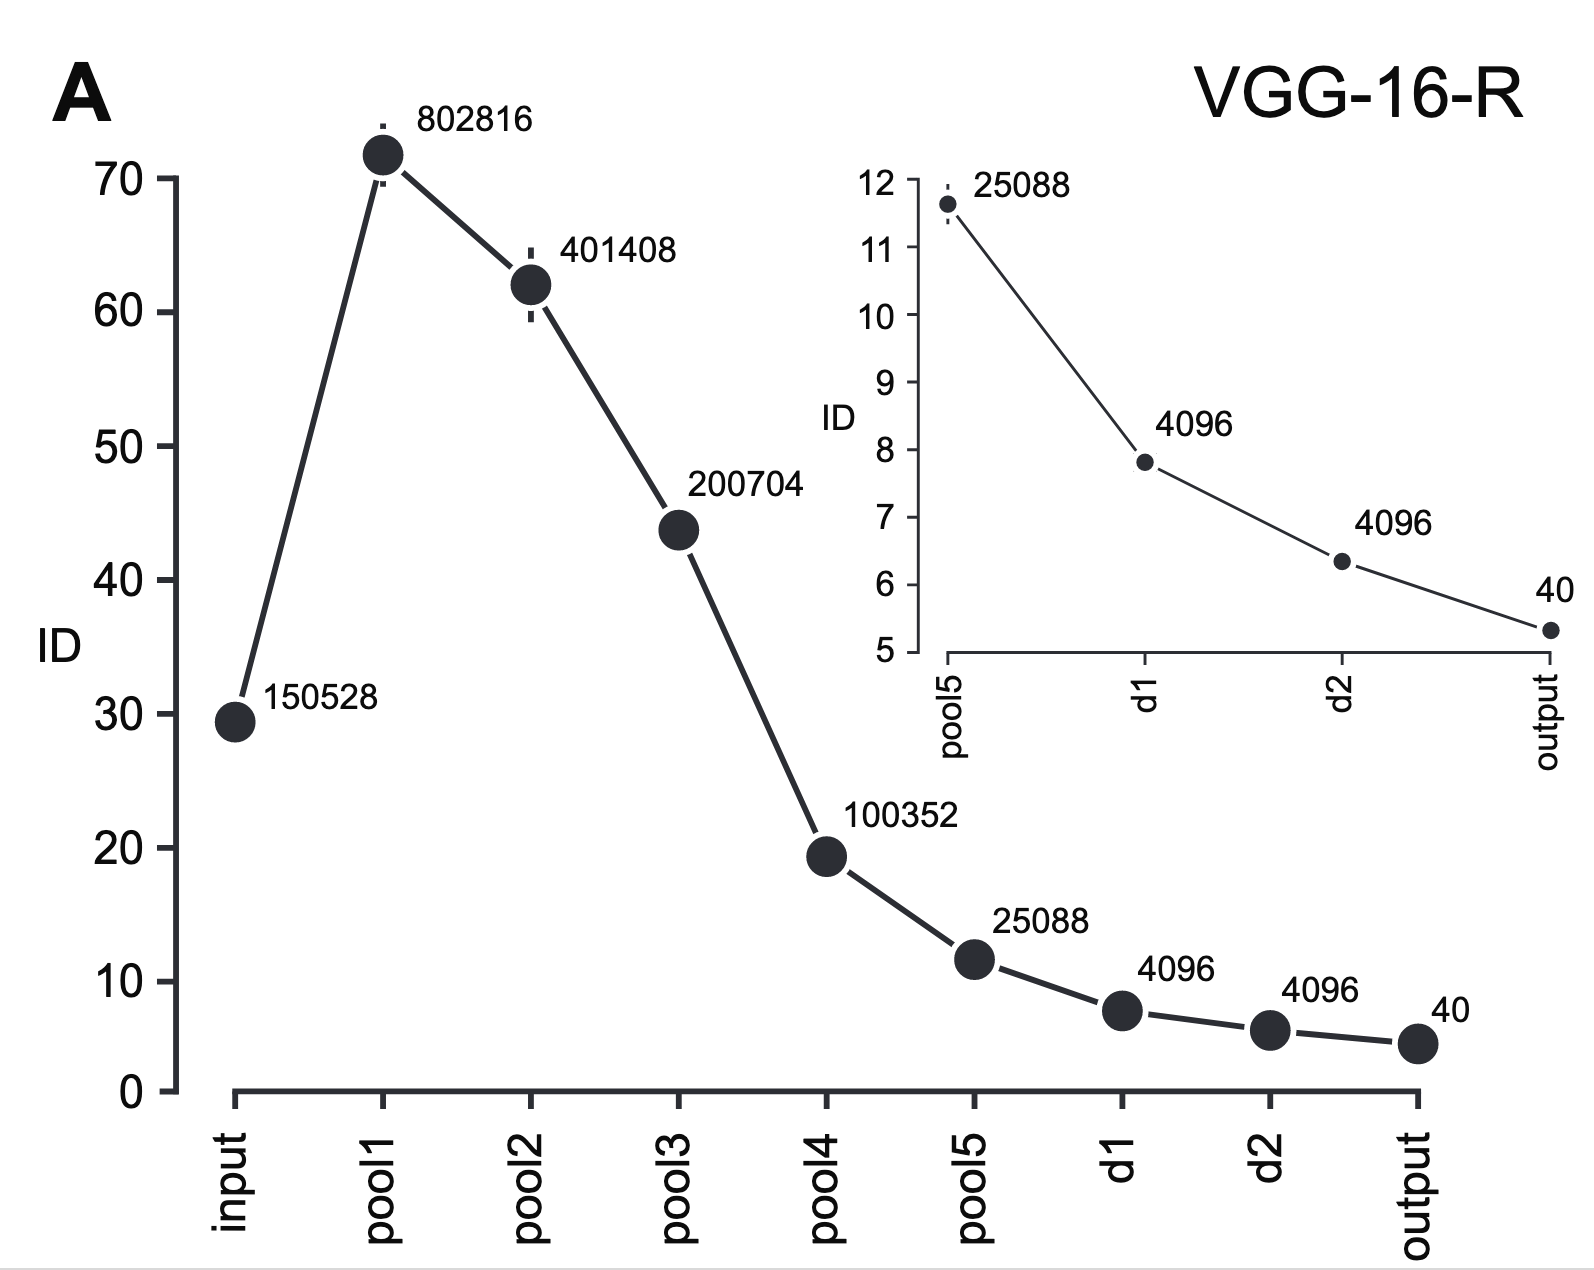
\includegraphics[width=0.5\linewidth]{profil Hunchback.png}
    \caption{Évolution de la Dimensionnalité Intrinsèque (ID) à travers les couches d'un réseau profond (VGG-16), illustrant le profil caractéristique « Hunchback » : une expansion suivie d'une compression. \textit{Source : Ansuini et al. [1]}}
    \label{fig:hunchback}
\end{figure}

Cela suggère que la performance d’un modèle provient de sa capacité à explorer la complexité d’un signal avant de le réduire en concepts abstraits de basse dimension.



\subsection{Mécanismes Prédictifs et ID}
Au-delà de l'observation, Recanatesi et al. (2021) lient l'émergence de ces structures de basse dimension au paradigme de l'apprentissage prédictif. Un point crucial soulevé par cette étude est la distinction entre deux types de mesures lors de l'apprentissage :

\begin{itemize}
    \item \textbf{La Dimensionnalité Linéaire (PR) :} Elle a tendance à augmenter ou rester élevée. Le réseau utilise un maximum d'espace pour "étaler" les représentations et les rendre facilement lisibles (linéairement séparables).
    \item \textbf{La Dimensionnalité Intrinsèque (ID non-linéaire) :} À l'inverse, celle-ci diminue drastiquement. C'est la preuve que les données, bien qu'étalées dans un grand espace, se concentrent sur une variété compacte.
\end{itemize}

Un gain élevé (rapport entre dimension linéaire et ID) signale que le modèle a construit une représentation robuste. Cela confirme que l'apprentissage prédictif force l'émergence de représentations structurées logiques, contrairement à d'autres méthodes comme l'auto-encodage simple.

% --- SECTION 1.3 ---
\section{Principes Neurolinguistiques et Parallèles IA}

Après avoir étudié les Transformers et l'ID, nous allons nous intéresser aux bases neurobiologiques du langage qui permettent au cerveau de construire le sens. Le traitement du langage par le cerveau est une fonction cognitive complexe impliquant de faire fonctionner ensemble la mémoire, l’attention et des processus combinatoires.

\subsection{Le Modèle MUC : Mémoire, Unification, Contrôle}
Le modèle dominant actuel est le \textit{Memory, Unification, and Control} (MUC) proposé par Peter Hagoort \cite{hagoort2013memory}. Il vient remplacer le modèle de Wernicke-Lichtheim-Geschwind, qui se focalise sur le mot unique. Le MUC structure le traitement linguistique en trois composantes distinctes mais interactives :

\begin{itemize}
    \item \textbf{Mémoire (Memory) :} C’est la composante qui va servir au stockage et à la récupération des connaissances linguistiques acquises (formes phonologiques, morphologiques, cadres syntaxiques). Elle est principalement localisée dans le cortex temporal gauche en jaune sur la Figure \ref{fig:muc_brain}.
    \item \textbf{Unification :} L'unification est l'assemblage dynamique des briques lexicales récupérées en mémoire pour former des structures cohérentes. Ce processus se déroule principalement dans le gyrus frontal inférieur gauche (aire de Broca) représentée en bleu sur la Figure \ref{fig:muc_brain}. C'est ici que la syntaxe et la sémantique fusionnent pour construire une représentation unifiée. 
    \item \textbf{Contrôle (Control) :} Cette composante gère l'attention, le tour de parole et la sélection de la langue pertinente, impliquant le cortex préfrontal dorsolatéral en rose sur la Figure \ref{fig:muc_brain}.
\end{itemize}

\begin{figure}[H] % On remplace [htbp] par [H]
    \centering
    % Remplacez 'nom_de_l_image_cerveau' par le vrai nom du fichier
    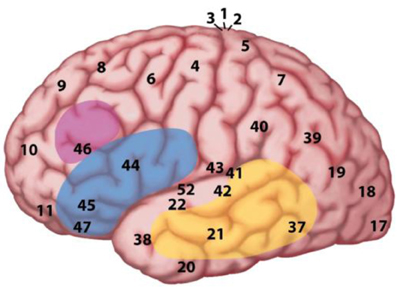
\includegraphics[width=0.5\textwidth]{The-MUC-model-of-language-The-figure-displays-a-lateral-view-of-the-left-hemisphere-The.png}
    
    % La légende simplifiée pour aller à l'essentiel
    \caption{Localisation anatomique des composantes du modèle MUC dans l'hémisphère gauche. En jaune : la Mémoire (cortex temporal). En bleu : l'Unification (aire de Broca). En rose : le Contrôle (cortex préfrontal). \textit{Source : Hagoort [5]}}
    
    \label{fig:muc_brain}
\end{figure}

L’unification implique que le cerveau maintient une représentation active qui croît en complexité à mesure que de nouveaux mots sont intégrés. Cette charge cognitive croissante devrait, selon notre hypothèse, se refléter dans la dimensionnalité de l'activité neuronale (et artificielle).

\subsection{Signatures Dynamiques : Le "Ramping" et l'Intégration}
Des études récentes (Fedorenko et al., 2016 \cite{fedorenko2016broad} ; Desbordes et al., 2023 \cite{desbordes2023}) ont identifié des marqueurs temporels de cette unification : l'activité de \textit{ramping}, une augmentation lente et continue de la puissance neuronale au cours de la phrase.

Ce signal ne répond pas simplement à chaque mot individuellement (activité phasique), mais semble accumuler l'information contextuelle. Les expériences utilisant des paradigmes "Jabberwocky" (phrases syntaxiquement correctes mais sans sens) révèlent que si la structure syntaxique seule crée une activité, les phrases sensées génèrent un \textit{ramping} beaucoup plus soutenu. Ce phénomène est également observé par Desbordes et al. (2023) dans les modèles artificiels.

% --- SECTION 1.4 ---
\section{Synthèse et Hypothèses de Travail}

En croisant ces trois domaines (Transformers, ID, Neurolinguistique), nous formulons les hypothèses qui guideront notre méthodologie pour la suite de ce projet :

\begin{enumerate}
    \item Les modèles de langage, comme le cerveau, présentent une activité de \textit{ramping} au cours de la lecture d'une phrase.
    \item La dimensionnalité intrinsèque des représentations augmentera plus fortement pour les phrases sémantiquement cohérentes que pour les phrases Jabberwocky, reflétant le coût computationnel de l'unification sémantique.
    \item Le profil de l'ID à travers les couches des Transformers montrera une expansion suivie d'une compression (profil \textit{Hunchback}), mais cette dynamique sera perturbée par les stimuli Jabberwocky, le modèle échouant à converger vers une représentation stable faute de sens.
\end{enumerate}

% --- CONCLUSION DU CHAPITRE (OBLIGATOIRE) ---
Dans ce chapitre, nous avons posé les bases théoriques liant l'architecture des Transformers aux théories neurolinguistiques via l'analyse de la dimensionnalité intrinsèque. Ces éléments constituent le fondement de notre approche expérimentale, dont nous détaillerons la méthodologie et l'implémentation dans le chapitre suivant.